\documentclass[12pt]{book}
\renewcommand{\figurename}{Imagen}
\usepackage{graphicx}
\begin{document}
\begin{figure} 
\begin{center}
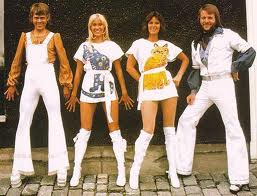
\includegraphics{ABBA.jpg}
	\end{center}
\caption{Portada de Disco Voulez-Vous}	
\label{Figura_ABBA} 
\end{figure}
En la imagen \ref{Figura_ABBA}, se observa 
la portada un disco de ABBA. 
\begin{figure} 
\begin{center}
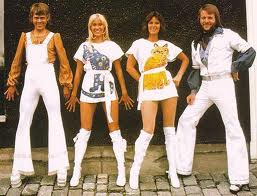
\includegraphics[scale=0.8]{Praga.jpg} 
\end{center} \caption{Vista de Praga}	
\label{Figura_Praga} 
\end{figure}
En la figura \ref{Figura_Praga}, se observa 
el castillo de Praga al fondo. 
\end{document}
